\documentclass{article}
\usepackage{amsmath}
\usepackage{amssymb}
\usepackage{graphicx}
\usepackage{hyperref}
\usepackage[version=4]{mhchem}

\title{Problem 7}
\date{}

\begin{document}
\maketitle

\section*{Problem}
As shown in the figure, circle \(K\) has diameter \(A B\); circle \(L\) is tangent to circle \(K\) and to \(A B\) at the center of circle \(K\); and circle \(M\) is tangent to circle \(K\), to circle \(L\) and to \(A B\). Find the ratio of the areas of circles \(K, L, M\).\\
\centering
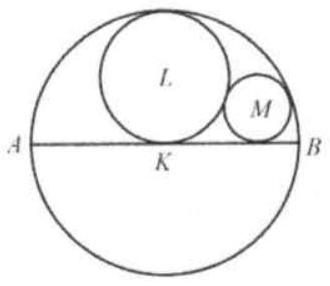
\includegraphics[width=\textwidth]{images/problem_image_1.jpg}

\section*{Solution}
16:4:1.
\(M F\) is parallel to \(A B\) and intersects \(K L\) at \(F\). Let \(r, s(=r / 2)\) and \(t\) be the radii of the circles with centers \(K, L\) and \(M\), respectively. Using the Pythagorean theorem to \(\triangle F L M\) and \(\triangle F K M:(M F)^{2}=\left(\frac{r}{2}+t\right)^{2}-\left(\frac{r}{2}-t\right)^{2}\), \((M F)^{2}=(r-t)^{2}-(t)^{2}\).\\
Solving w get \(r: t=4: 1\). So \(r: s: t=4: 2: 1\).\\
The ratio of the areas is then is \(16: 4: 1\).\\
\centering
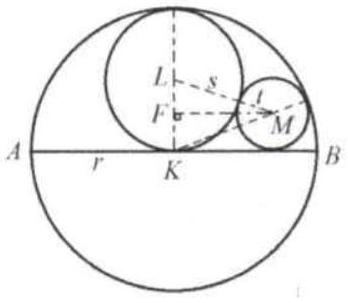
\includegraphics[width=\textwidth]{images/reasoning_image_1.jpg}

\end{document}
